\section{Week 4: 2nd - 8th February 2026}

\subsection{Thursday 5th February}

\subsubsection{Meeting 4: Zhaoting and Alkistis}

Since our last meeting I mainly just reviewed the code that I had written and tried to connect what I did there to the theory I read in the papers.

\begin{itemize}
    \item Went over the significance of why removing low values of k para affects the data so much.
    \begin{itemize}
        \item Small k para relates to the very high frequency values. This relates to the smooth foreground we want to remove.
        \item The small eigenvalues of the signal relate to the modes. The smallest modes correspond to the foreground.
    \end{itemize}
\item If we add polarised foregrounds to the smooth foregrounds, if we remove the small modes, we will remove the smooth foregrounds but also some of the polarised foregrounds.
\item The more k para and modes we remove, the closer our data will look to the signal since our HI signal has very large modes and is very oscillatory. However, that mean we will be increasing the amount of signal we are removing.
\item We want to make sure to balance the amount of foreground and noise we are removing with the amount of signal we are keeping. 
\item With PCA, we are just manually looking at which modes and k values correspond to what frequencies. With GPR, we will be fitting kernels to as closely mimic our foreground and noise and signal. We mainly just want to closely match the covariance.
\item Our next meeting will be on Tuesday at 11am on Zoom only with Zhaoting since Alkistis is not available.
\begin{itemize}
    \item Zhaoting will send me notebook 3 with the next steps of the project and will start on GPR and fitting different kernels to try to match our foregrounds and signals. He will send me this on Monday.
    \item Over the weekend, I should try to extract the eigenvectors instead of eigenvalues. This will help me better visualise and understand how the eigenvalues/eigenvectors connect with the frequencies and modes, etc. I should also try to plot the cylindrical power spectrum with the foreground signal or noise (which is generated by using np.gaussian.random I think). This is just to better understand how the cylindrical power spectrum relates to the frequencies and signals.
\end{itemize}
\end{itemize}

To do before Monday:

\begin{itemize}
    \item From notebook 2:
    \begin{itemize}
        \item Extract the eigenvectors and try to understand what it shows and why it's significant.
        \item Plot the cylindrical power spectrum for the foreground noise and gaussian noise and try to understand what it shows and why it's significant.
    \end{itemize}
\end{itemize}

Sunday 8th February

\begin{figure}[hbt!]
    \centering
    
\includegraphics[width=0.75\linewidth]{outputs//week4/eigenvalues.pdf}
    \caption{Eigenvalues of the total signal. We can see the first 3 [0, 1, 2] modes are very large and then it plateaus. These correspond to the foregrounds.}
    \label{fig:placeholder}
\end{figure}

\begin{figure}[hbt!]
    \centering
    
\includegraphics[width=0.75\linewidth]{outputs//week4/eigenvectors.pdf}
    \caption{Eigenvectors of the total signal. We can see the first 2 [0, 1] modes are very smooth which is expected from the foreground signal. The rest of the modes [3-9] become increasingly "wiggly" which represent higher frequency fluctuations.}
    \label{fig:placeholder}
\end{figure}

Instructions from an email sent on Thursday which has different code snippets

\begin{itemize}
    \item Some stuff you can plug into the previous notebook. In the previous notebook there is this part:
    \begin{itemize}
        \item tot\_map = hi\_map + fg\_map
        \item cov\_matrix, \_, eigen\_values, \_, = pca\_clean(tot\_map,1,weights=mock.w\_HI,return\_analysis=True,mean\_center=True)
    \end{itemize}
\item You can change that to:
\begin{itemize}
    \item sigma\_noise = 1.21 * 1e-3
    \item noise\_map = np.random.default\_rng(mock.seed).normal(0,sigma\_noise,hi\_map.shape) * mock.w\_HI
    \item tot\_map = hi\_map + fg\_map + noise\_map
    \item cov\_matrix, \_, eigen\_values, eigen\_vectors, = pca\_clean(tot\_map,1,\textit{weights}=mock.w\_HI,\textit{return\_analysis}=True,\textit{mean\_center}=True)
    \item \textit{\# plot the first 10 eigenvectors}
    \item fig,axes = plt.subplots(10,1,\textit{figsize}=(10,8))
    \item \textit{for} i \textit{in} range(10):
    \item axes[i].plot(eigen\_vectors[:,i])
    \item plt.show()
\end{itemize}
\item Here I am doing two things, adding in a noise component and also plotting the eigenvectors.
\item Later in the notebook there is this part:
\begin{itemize}
    \item mock.data = hi\_map
    \item mock.grid\_data\_to\_field();
    \item power\_cy\_hi,\_ = mock.get\_cy\_power(mock.auto\_power\_3d\_1)
    \item power\_1d\_hi,k\_1d,nmodes\_1d = mock.get\_1d\_power(mock.auto\_power\_3d\_1)
    \item mock.data = res\_map
    \item mock.grid\_data\_to\_field();
    \item power\_cy\_res,\_ = mock.get\_cy\_power(mock.auto\_power\_3d\_1)
    \item power\_1d\_res,k\_1d,nmodes\_1d = mock.get\_1d\_power(mock.auto\_power\_3d\_1)
\end{itemize}
\item Simply change the input data to fg\_map or noise\_map and you can calculate the foreground power and noise power.
\end{itemize}

Working more on notebook 2 and doing what was mentioned during Thursday's meeting

\begin{itemize}
    \item Extract the eigenvectors and try to understand what it shows and why it's significant
    \begin{itemize}
        \item The plot of the eigenvalues can be seen in Figure 25. This was generated last week but is shown here again for better compare with the eigenvector plots.
        \begin{itemize}
            \item We can see the first 3 [0, 1, 2] modes are very large and then it plateaus. These correspond to the foregrounds.
            \item This plot shows us how much power a component has.
        \end{itemize}
        \item The plot of the eigenvectors can be seen in Figure 26. 
        \begin{itemize}
            \item We can see the first 2 [0, 1] modes are very smooth and linear which is expected from the foreground signal. This is because the synchrotron radiation is very bright and vary very slowly across frequency.
            \item The rest of the modes [3-9] become increasingly "wiggly" which represent higher frequency fluctuations.
            \item This plot shows us what the power/mode looks like across the frequency ranges.
            \item These very wiggly lines are much lower in magnitude than the foregrounds and vary a lot from frequency-to-frequency.
        \end{itemize}
    \end{itemize}

\begin{figure}[hbt!]
    \centering
    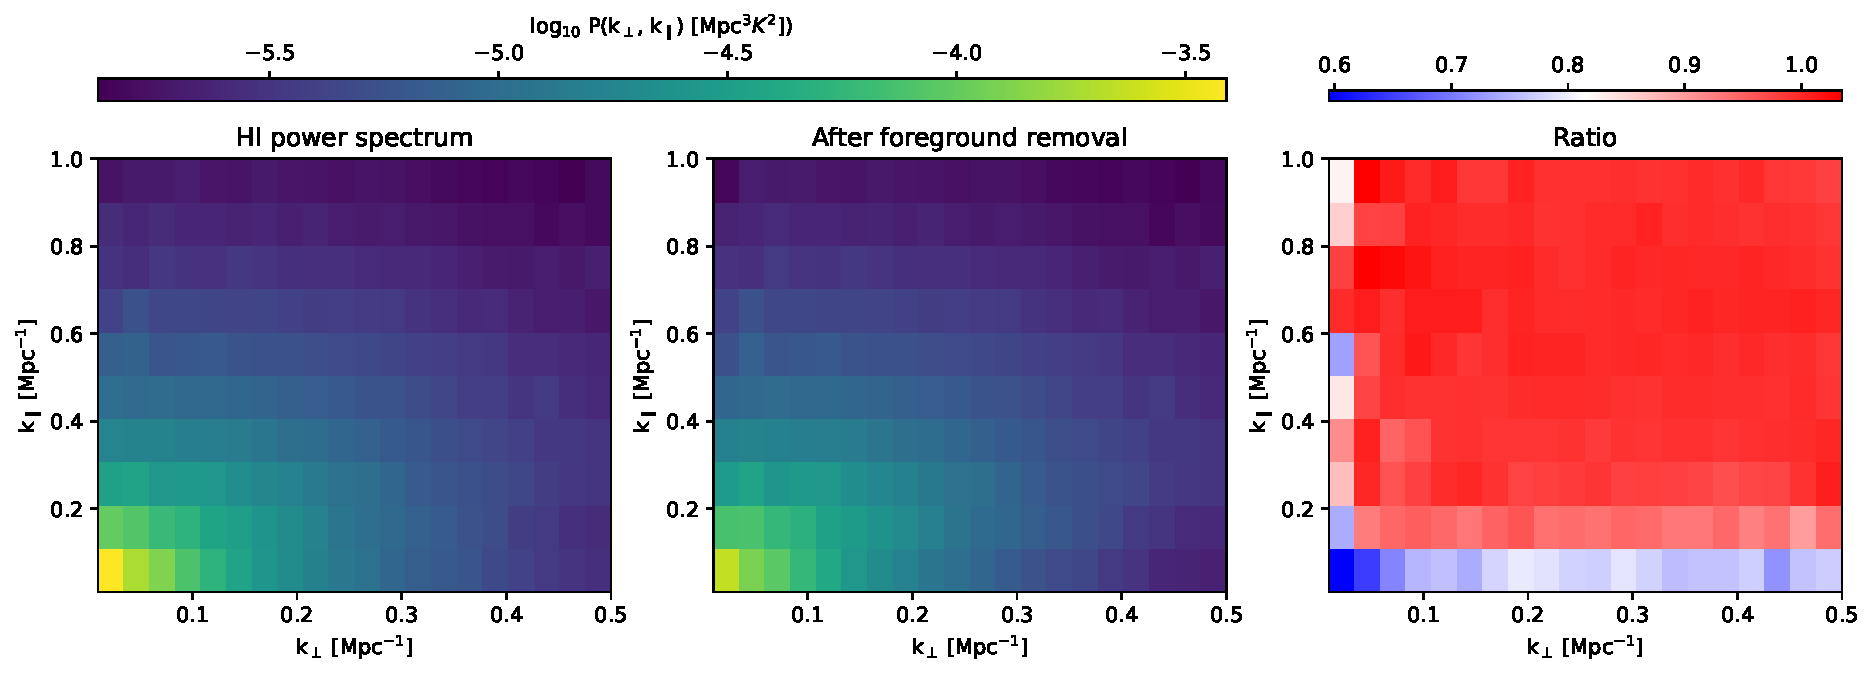
\includegraphics[width=0.8\linewidth]{outputs/week4/cylindrical_power_spectrum_hi_map.pdf}
    \caption{The cylindrical power spectrum of the HI signal.}
    \label{fig:placeholder}
\end{figure}

\begin{figure}[hbt!]
    \centering
    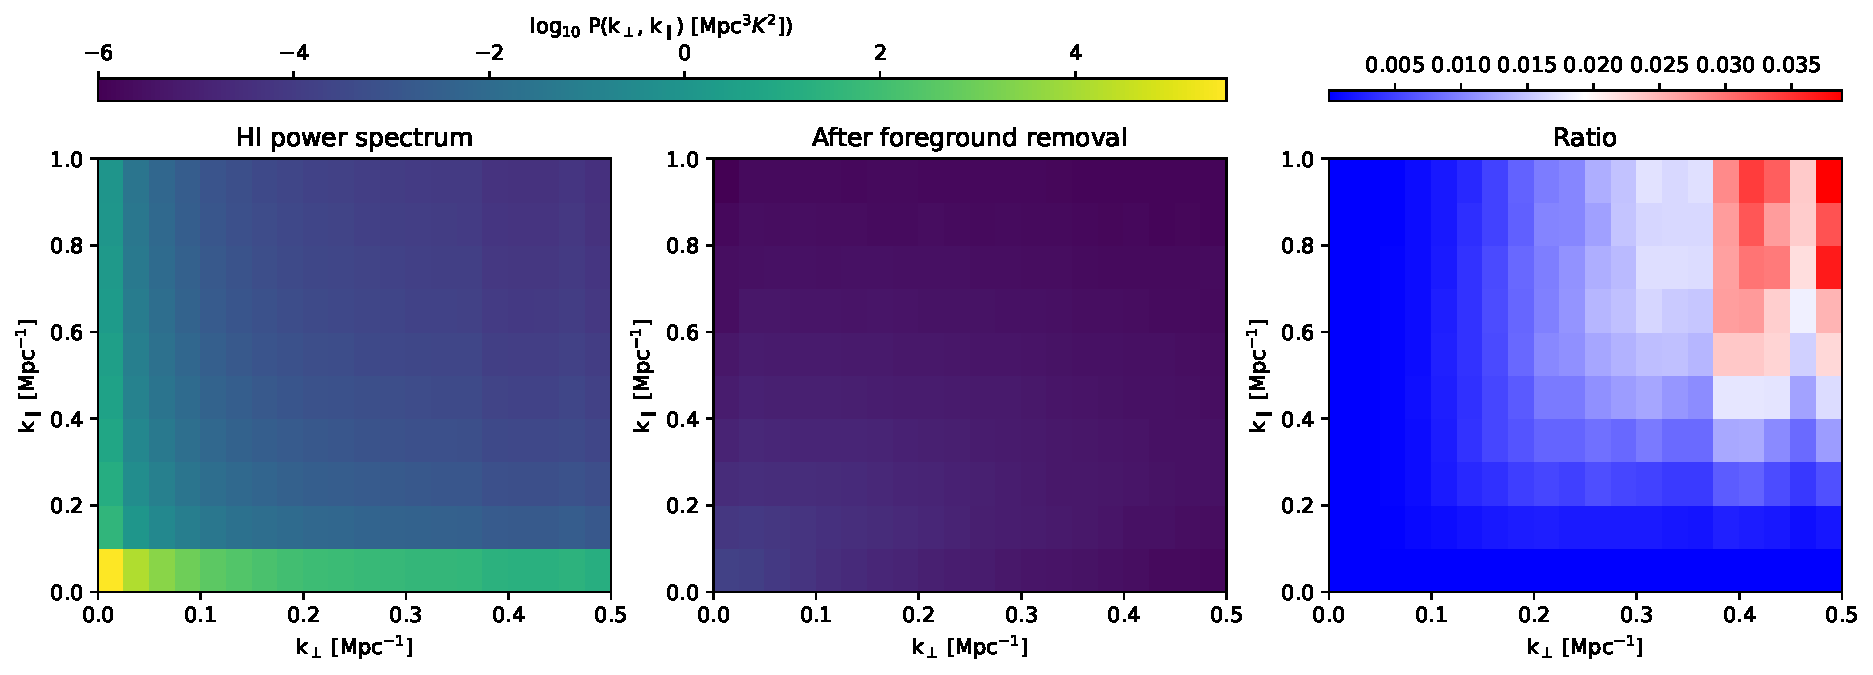
\includegraphics[width=0.8\linewidth]{outputs//week4/cylindrical_power_spectrum_fg_map.pdf}
    \caption{The cylindrical power spectrum of the foreground.}
    \label{fig:placeholder}
\end{figure}

\begin{figure}[hbt!]
    \centering
    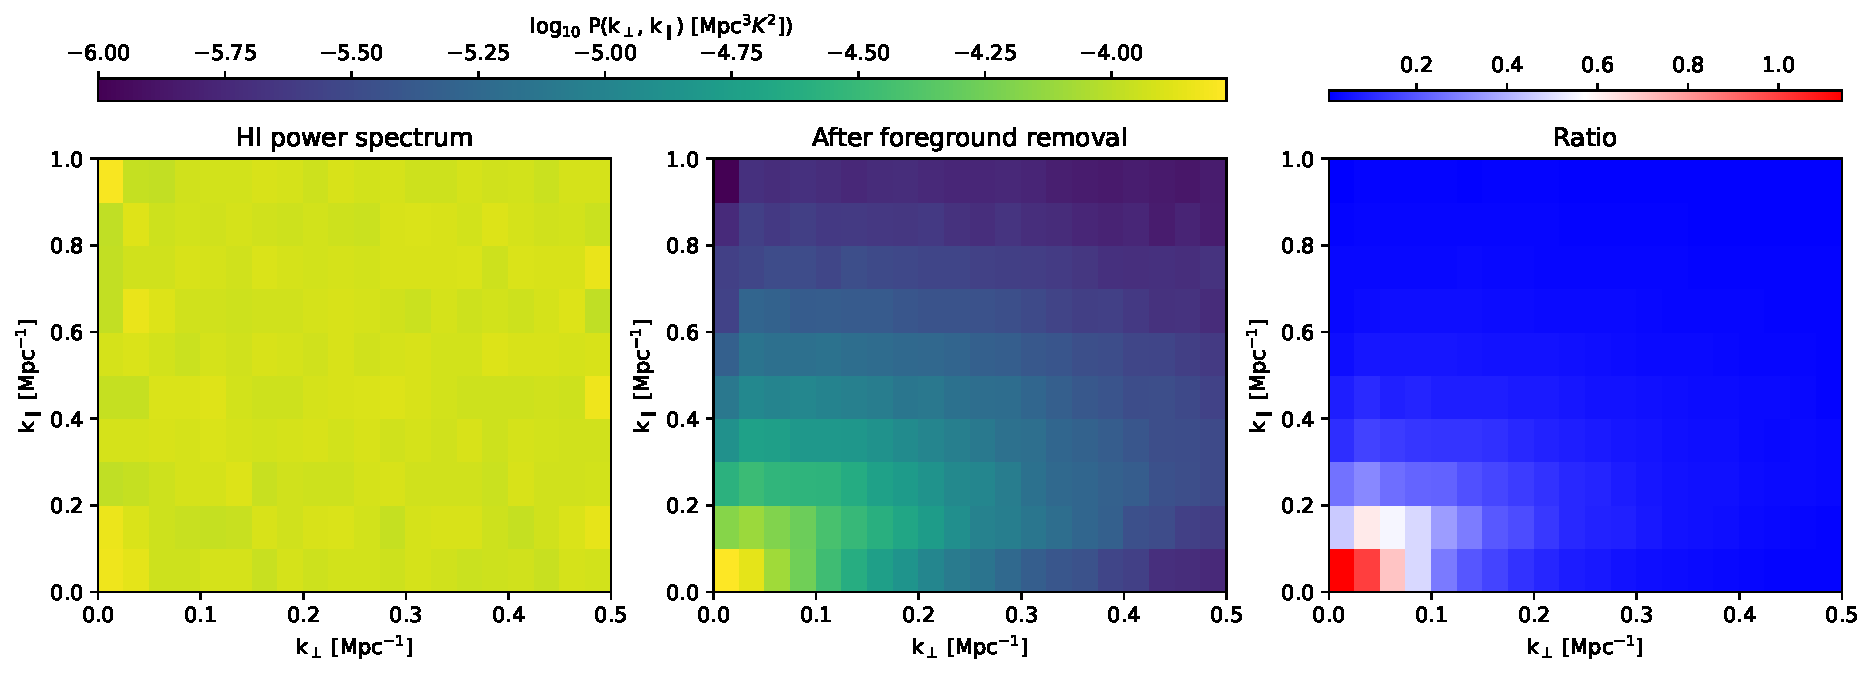
\includegraphics[width=0.8\linewidth]{outputs//week4/cylindrical_power_spectrum_noise_map.pdf}
    \caption{The cylindrical power spectrum of the noise. }
    \label{fig:placeholder}
\end{figure}
    
    \item Plot the cylindrical power spectrum for the foreground noise and Gaussian noise and try to understand what is shows and why it's significant.
    \begin{itemize}
        \item The cylindrical power spectrum of the HI signal (generated last week) can be seen in Figure 27.
        \begin{itemize}
            \item After foreground removal shows a significant drop in power.
            \item The ratio plot shows the most signal loss occurs at low k para. 
            \item This is because the HI signal has some large-scale structures that is smooth which partially overlaps with the foreground modes. When PCA removes the first few eigenvectors, it cannot distinguish between smooth foregrounds and smooth HI signal.
        \end{itemize}
        \item The cylindrical power spectrum of the foreground can be seen in Figure 28.
        \begin{itemize}
            \item Before removal, the power is almost entirely concentrated at low k para which is expected as it represents the smoothness of the foreground.
            \item After foreground removal, the plot is almost completely dark showing that the PCA modes that were selected and removed match the foreground shapes well.
            \item The red region at high k in the ratio map suggests that while most of the power was removed, small-scale residuals or noise might still remain.
        \end{itemize}
        \item The cylindrical power spectrum of the noise can be seen in Figure 29.
        \begin{itemize}
            \item This was done by generating Gaussian white noise which represents the thermal noise of the instrument.
            \item The noise power spectrum is relatively uniform across the entire k para k perp plane. This is what is expected from white thermal noise.
            \item The after foreground removal looks very similar to the HI power spectrum after foreground removal. 
            \item The ratio plot looks almost reversed in comparison to the HI signal ratio. Suggesting signal loss occurs everywhere except low k para and low k perp?
        \end{itemize}
    \end{itemize}
\end{itemize}

\subsection{Wednesday 11th February}

To-do list for today (and/or the rest of the week):
\begin{itemize}
    \item I will try to get as much of the following done:
    \item Update lab book with meeting notes from yesterday
    \item Look at code for the cylindrical power spectrum and try to understand the issue. Also try to fix it and do the correct plots.
    \item Download the new GPR notebook and have a look. 
    \item And make notes in my lab book on any of the tasks completed.
\end{itemize}